% iaus2esa.tex -- sample pages for Proceedings IAU Symposium document class
% v1.04,  Copyright (2004) International Astronomical Union

\NeedsTeXFormat{LaTeX2e}
\newcommand{\squeezeup}{\vspace{-1.5mm}}

\documentclass{iau}
% Include figures (EPS only), using e.g.:
\usepackage{graphicx,float}
\floatplacement{figure}{H}



%% -- Title ------------------------------------
\title[Multiwavelngth Astronomy ~~PSR J0737$-$3039] %% short title %%
{A Multiwavelength Review of PSR J0737$-$3039} %% full title %%

%% -- Authors ----------------------------------
\author[Umang Mishra]  %% short author list %%
{Umang Mishra $^1$}
% \thanks{Present address: ...},
%% \and Author Two$^2$}

\affiliation{New York University Abu Dhabi\\ email: {\tt um339@nyu.edu}} 
%%\\[\affilskip]
%%$^2$A, \\ B \\email: {\tt c@d.com}}

%% -- Header (pre-filled, do not edit) -----------------
%\pubyear{2012}
%\volume{1}  %% insert here IAU Symposium No.
% \pagerange{1--9}
% \date{?? and in revised form ??}
% \setcounter{page}{1}
%\jname{\mbox{Multi-Wavelength Astronomy: Final Reports of Sources Studied in Depth}}
%\editors{M. S. E. Roberts , ed.} 
\begin{document}

\maketitle

%% -- Abstract ----------------------------------
\begin{abstract}

This paper presents a multi-wavelength review of the double neutron star system PSR J0737-3039. Since its discovery in 2004, the system has been extensively studied in radio and X-ray spectrum. There have also been attempts to observe the source in Optical but only constraints could be obtained with no observations. PSR J0737-3039 has given one of the best tests for general relativity and proved to be a unique testing ground to study pulsar magnetospheric interactions. This review aims to give an overview of the radio, X-ray, optical and ultraviolet observations of the system and how they gave us a better understanding of the system, while posing some new questions about magnetic wind interactions between the pulsars. The more recent gamma ray observations are also discussed.

%% add here a maximum of 10 keywords, to be taken form the file <Keywords.txt>
\keywords{PSR J0737$-$3039,Double Pulsar Binary, General Relativity}
\end{abstract}

% add below any authors, subjects and objects for indexing 
%   add more lines if necessary
%   but leave all lines commented out
%\index[author]{LastName1, Initials|textbf}
%\index[author]{LastName2, Initials|textbf}
%\index[subject]{Keyword1}
%\index[subject]{Keyword2}
%\index[object]{Object1}
%\index[object]{Object2}


\firstsection % if your document starts with a section,
              % remove some space above using this command.
\section{Introduction}

The first binary radio pulsar to be discovered was the Hulse-Taylor binary system. Since then, 15 such systems have been discovered. While most of the pulsars in doble neutron stars are recycled pulsars, the DNS systems PSR J0737-3039 and PSR J1906+0746 host pulsars which do note seem to have evolved as a recycled pulsar. In fact, up until very recently, PSR-J0737-3039 was the only system where both the neutron stars were observed as pulsars. 

Right from its discovery, the pulsar binary was anticipated to be crucial towards better understanding of  Post Newtonian formalism and gravitational waves. J0737$-$3039A is a millisecond pulsar with 22.7ms period, and its counterpart is a young unrecycled pulsar with a period of 2.77 s as summarized by \cite{lyn06} . While initially the system was only observed in the radio wavelengths for testing general relativity, observations were also performed using Chandra XMM Newton in X-rays. The X-ray observations gave a more detailed understanding of the magnetospheric emissions in the system. However, there was a lot of debate about the emissions following a composite spectrum model involving a power law and blackbody component or just blackbody components.

To get a better understanding, observations in optical and ultraviolet spectrum were also performed which helped in providing better constraints on the emission model of the system. Furthermore, pulsar A was also observed more recently in gamma rays and helped confirm previous predictions about the system. 

\section{Radio Observations}

\subsection{The Discovery and the Parameters}
Although the first observation was made by the Parkes 64-m at 1390Hz, better precision was obtained after interferometric observations were made using the Australia Telescope Compact Array(ATCA). The pulsar A of the system was found to be in a 2.4 hour eccentric orbit with eccentricity of 0.088 by \cite{b03}. The ATCA measurements helped further measurement of parameters, giving a period of 22.699 ms for pulsar A. The period of pulsar B was found to be 2.8s by \cite{lyn04}.
 
The periastron advance($\dot\omega$) value was measured to be 16.88yr$^{-1}$. This was the highest value of $\dot\omega$ and was used to predict the masses of the pulsars in the system.\cite{lyn04} also measured other post Keplerian parameters, and found that the predictions of masses were accurate. The system was thus established as a highly relativistic double pulsar binary system ideal for testing relativistic gravity and DNS merger rates.

\subsection{The Double Neutron System(DNS) as a Testing Ground for General Relativity}

\begin{figure}[H]
	\begin{center}
		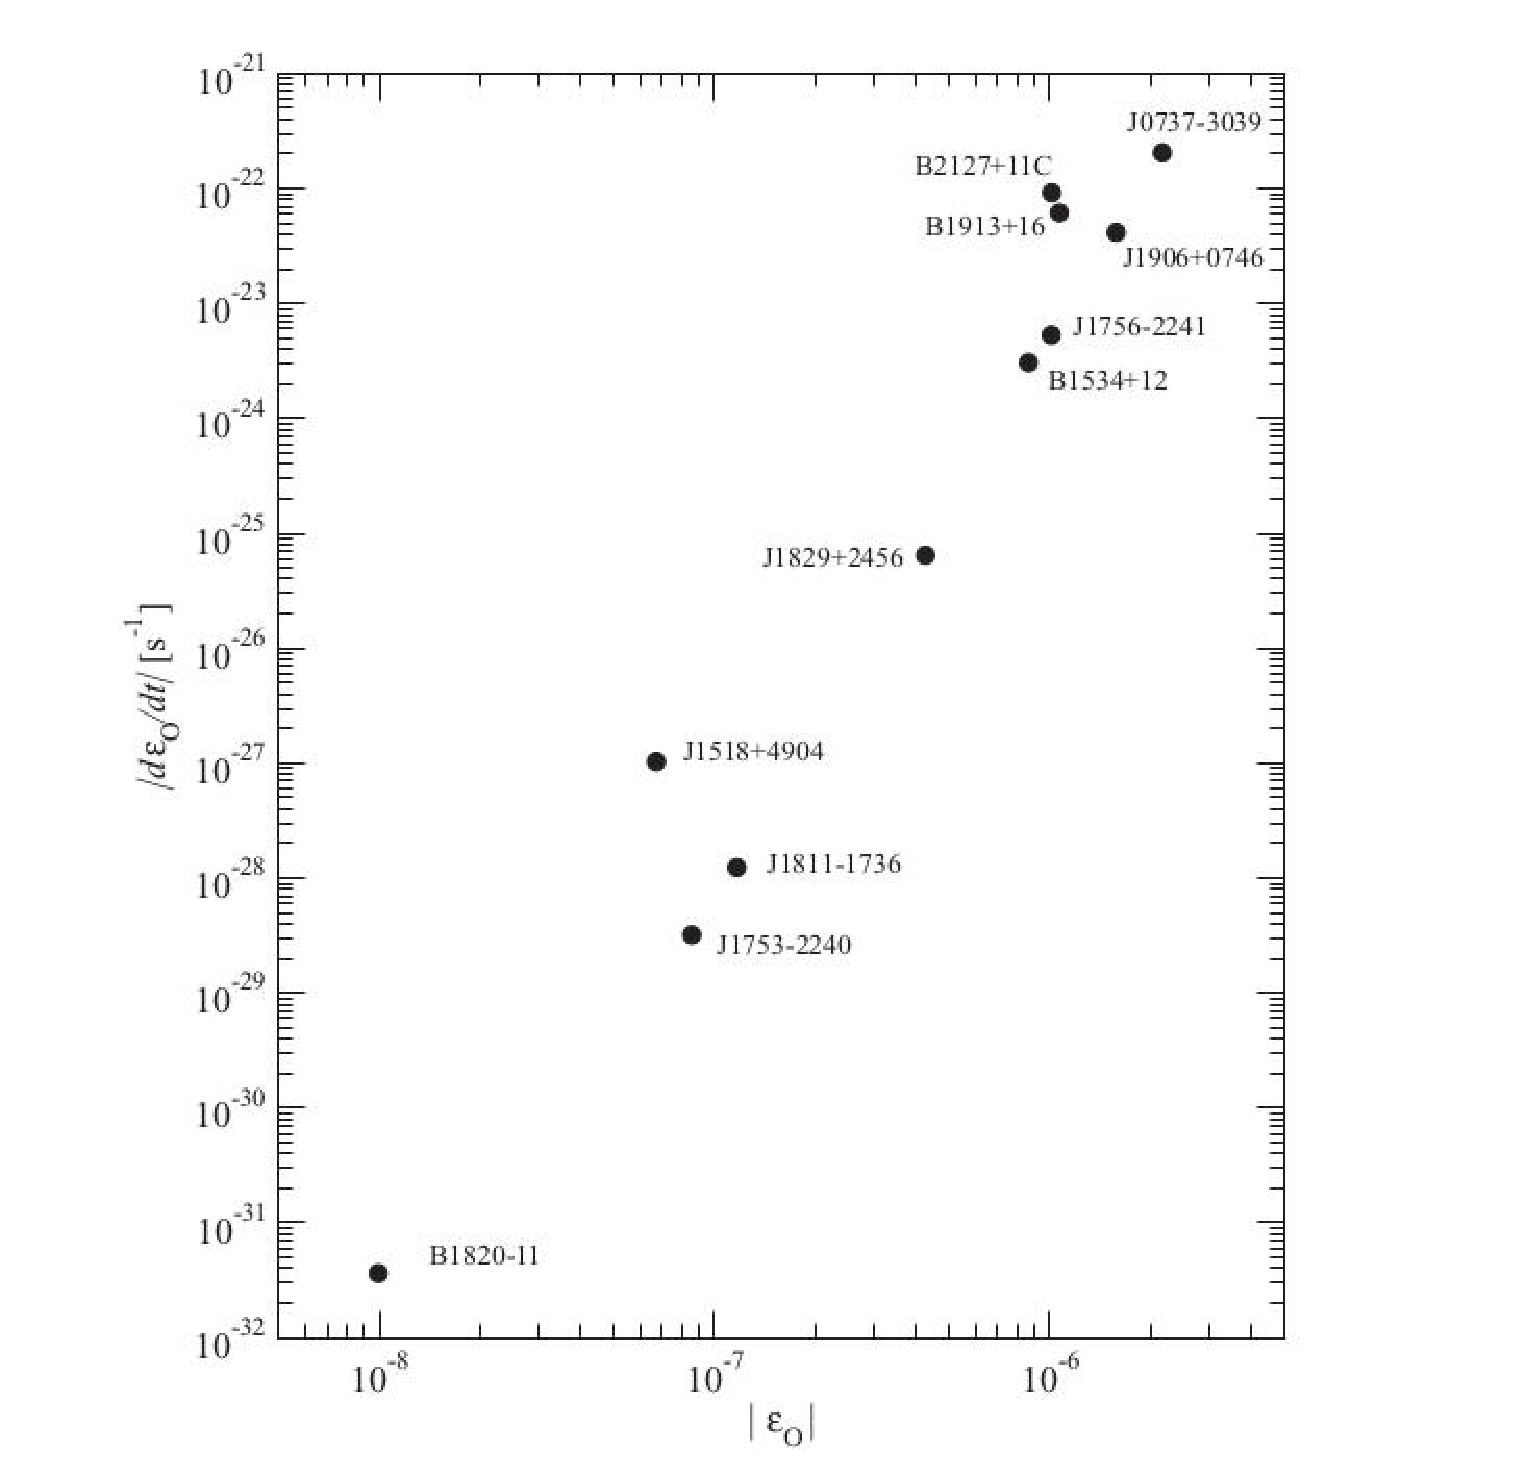
\includegraphics[width=3.4in]{fig1.eps} 
		\caption{Orbital energy-energy loss diagrams for known and likely double neutron binaries. $\epsilon_o$ is a direct measure for the strength of post-Newtonian effects in orbital dynamics. It can thus clearly be seen that J0737-3039 (top right) is the most suitable candidate for studying relativistic gravity. Image taken from \cite{kwex09} }
		\label{fig1}
	\end{center}
\end{figure}

Usually, five Keplerian Parameters are sufficient to describe binary systems. These are: P$_{orb}$, e, $\omega$, a$sin i$, and T$_o$. In case of strong gravitational interactions, such as in the case of a double neutron system, six additional parameters called the post-Keplerian parameters are required to fully describe the system due to relativistic effects that come into play. These are : $\dot\omega$, $\gamma$, $r$, $s$,dP$_b$/dt, and $\Omega_{SO}$. Since gravity is the only way stars in DNS interact, it makes them ideal candidates for studying relativistic gravity theories using these post-Keplerian parameters. The description of these parameters can be found in table 1. 

\begin{table}[]
	\centering
	\caption{A description of the six post-Keplerian parameters}
	\begin{tabular}{p{1cm}|p{3cm}|p{8cm}}
		\hline
		$\dot\omega$  & Periastron advance                     & Describes the rotation of the line connecting two pulsars at their closest approach to each other                        \\ \hline
		$\gamma$      & Gravitation Redshift and Time Dilation & Accounts for the apparent slowing of time due to general and special relativistic effects                                \\ \hline
		$r$ and $s$   & Shapiro Delay                          & These parameters define the Shapiro delay, which is delay in receiving signal due to space-time curvature                \\ \hline
		dP$_b$/dt     & Orbital Decay                          & The rate of decrease of the orbital period due to emission of gravitational waves                                        \\ \hline
		$\Omega_{SO}$ & Relativistic Spin Precession           & Rate of the apparent precession of the pulsar about the orbital angular momentum that arises due to space-time curvature \\ \hline
	\end{tabular}
\end{table}

As shown in figure 1, PSR J0737-3039 is the most suitable system for studying relativistic gravity.  Each of the post-Keplerian(PK) parameters is related to the masses of the pulsars in the system in a unique way.With a system as J0737-3039, a ratio of stellar masses can be obtained from observations and plotted as a straight line according to the equation: \[\frac{a_B sini}{a_A sini}=\frac{m_A}{m_b}\]
An intersection between this line and the curves plotted for each PK on a mass-mass plot could be used as a verification test for general relativity. 

In the case of PSR J0737-3039, all five PK parameters can be measured for pulsar A. Since the equations for $\dot\omega$, $s$, and dP$_b$/dt for general relativity are symmetric in masses, they will be the same for both pulsar A and pulsar B. Studies of eclipses of A allow for measurement of $\Omega_{SO}$ for B. The mass-mass plot for these parameters, can be seen in figure 2. While all the experimental values agree within the error boundaries with the theoretical predictions, the best match is with Shapiro delay(with uncertainty of 0.05\%). Exact values are listed in table 2. Since this was one of the only system where the angle of orbital inclination(i) was nearly edge on, it was the first time that Shapiro delay could be measured to such accuracy. It is also the first system where geodesic precession could be measured. The precession was measured in pulsar B by \cite{bret08}. The observed data is shown in figure 2. 

\begin{figure}[H]
	\begin{center}
		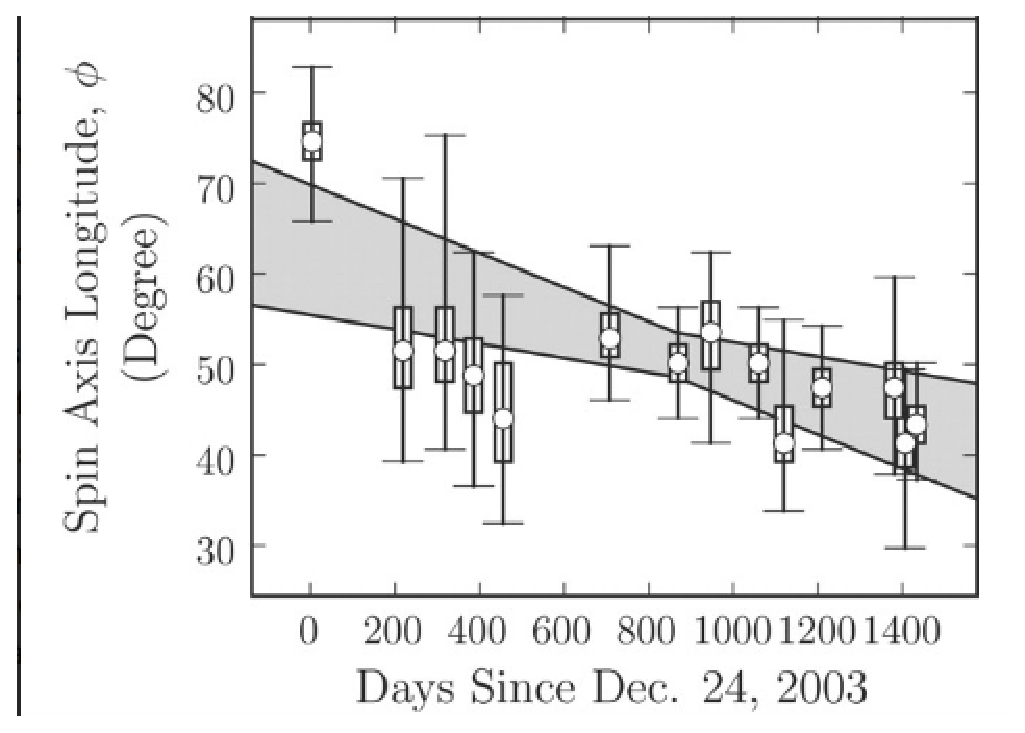
\includegraphics[width=3.4in]{fig14.eps} 
		\caption{Evolution of pulsar B's geometry as a function of time. For each data point, the circle represents the median value of the posterior probability density, whereas the box and the bar indicate the 1σ and 3σ confidence intervals, respectively. The gray regions are the 3σ confidence regions derived from the joint time-dependent model fitting. For clarity, multiple eclipses are displayed as single data points when observed over an interval of about a week. Taken from \cite{bret08}}
		\label{fig2}
	\end{center}
\end{figure}



\begin{table}[]
	\centering
	\caption{A comparison of measured and predicted values of the six post-Keplerian parameters. Values taken from \cite{kwex09}}
	\begin{tabular}{p{3cm} p{3cm} p{3cm} p{3cm}}
		\hline
		Parameter & Observed value & GR expectation & Ratio  \\ 
		\hline
		$\dot\omega$ (deg yr$^{-1}$)  &   (68) & - & -  \\ \hline
		$\gamma_A (ms) $     &  0.3856(26) & 0.38418(22) &  1.0036(68)   \\ \hline
		$r_A$ ($\mu$s)  & 6.21(33) &  6.153(26) & 1.009(55) \\ 
		\hline
		$s$  &0.999 74(−39, +16)&  0.999 87(−48, +13)&0.999 87(50) \\ 
		\hline
		dP$_b$/dt     & 1.252(17) & 1.24787(13) & 1.003(14)  \\ 
		\hline
		$\Omega_{SO}$ (deg yr$^{-1}$) & 4.77(+0.66, −0.65)  &  5.0734(7) & 0.94(13)  \\ \hline
	\end{tabular}
\end{table}


% CUP work flow only accepts EPS -- not PDF, JPG, etc.
\begin{figure}[H]
	\begin{center}
		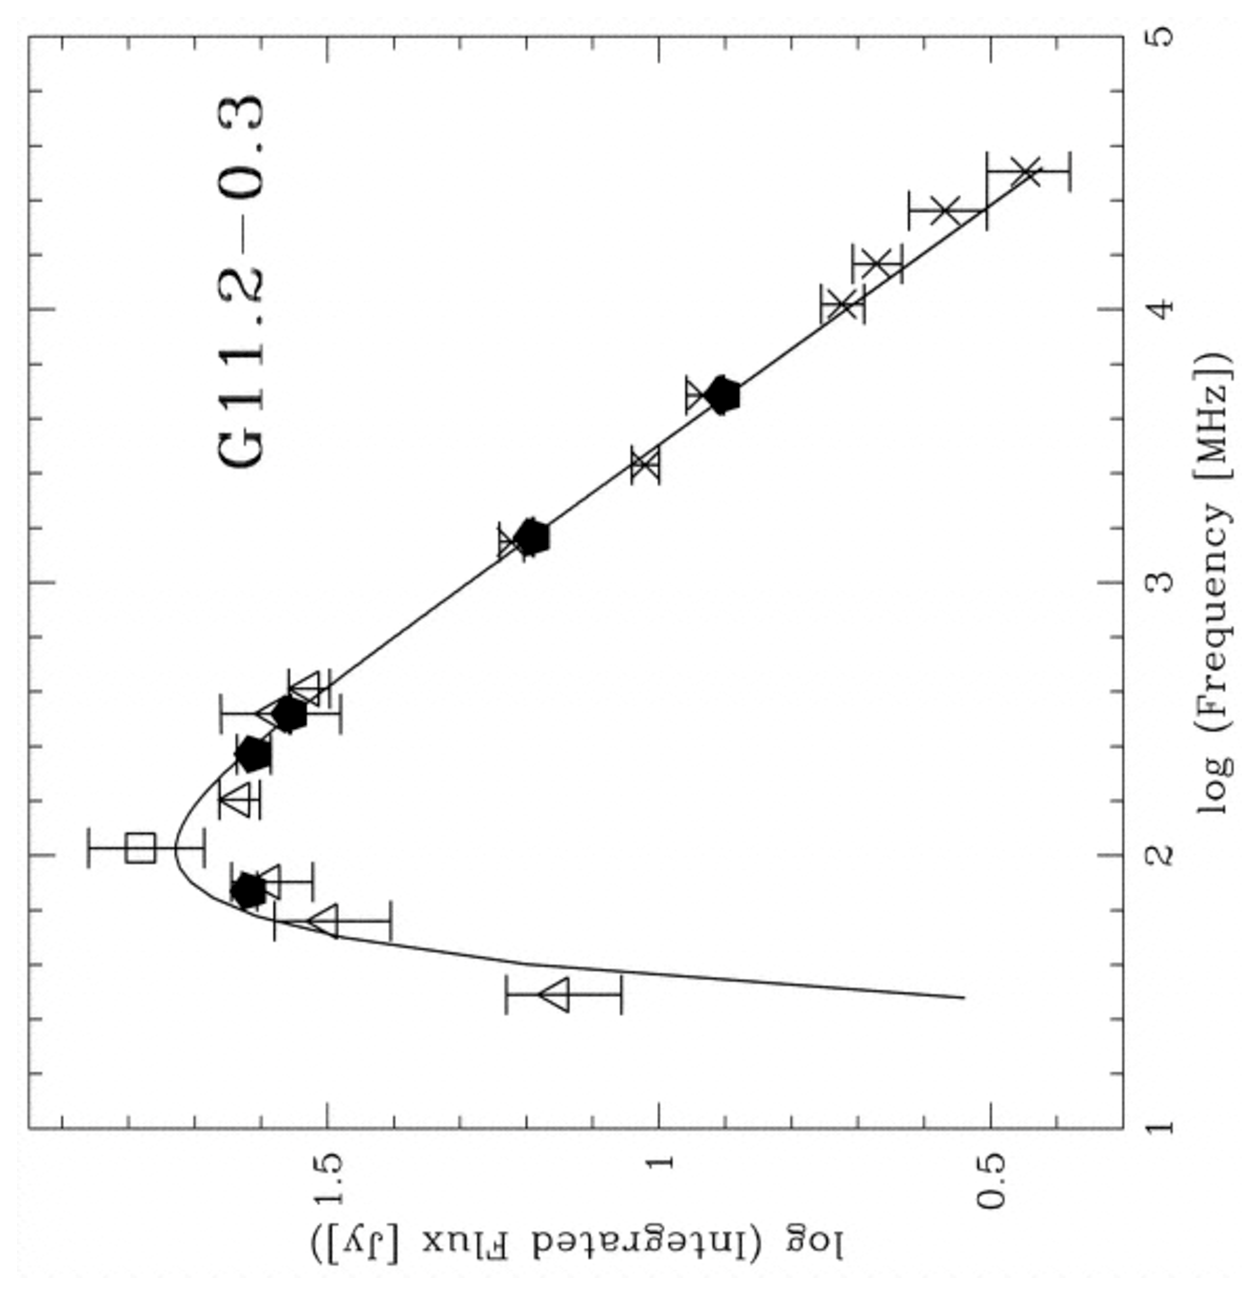
\includegraphics[width=3.4in]{fig2.eps} 
		\caption{M-M graph to test general relativity using PK parameters for PSR J0737-3039. Taken from \cite{james16}}
		\label{fig2}
	\end{center}
\end{figure}

 
\subsection{Eclipsing of A and the Penetration of B's Magnetosphere}

At conjunction, the line of sight of the two pulsars is within 0.15 ls of each other. As they further advance in their orbits, A is completely eclipsed by B and the line of sight of A sweeps through the magnetosphere of B. \cite{lyn04} suggested that studying the changes in radio transmission during this process can lead to understanding the physical conditions of B's magnetosphere, giving a better understanding of the plasma density and  magnetic field structure. Analysis of flux densities(figure 3) revealed an occultation of A occurs that lasts 30s. The spin-down energy loss of A being 3000 times greater than that of B, and the energy density of the relativistic wind from A being two orders of magnitude larger than B's, it was suggested that the wind from A will penetrate deep into B's magnetosphere. In fact, it was found that at radii greater than 40\% of the light cylinder of B, the energy field of A dominates. Because of this, the penetration of wind from A into that of B was hypothesized to be dependent on their relative orientation. This dependence was cited as the cause for fluctuations in B's flux densities over time. An accurate model was proposed by \cite{Lyut05} which perfectly predicted the eclipsing of A. The model clearly predicted the modulation of emission from pulsar during eclipse at half and full period of pulsar B. The model firmly established that neutron stars are surrounded by corotating, dipolar magnetic fields. It also gave an understanding of how pulsar magnetosphere interacts with external pulsar wind. The model superimposed on the observed eclipse profile is shown in figure 4. 

\begin{figure}[H]
	\begin{center}
		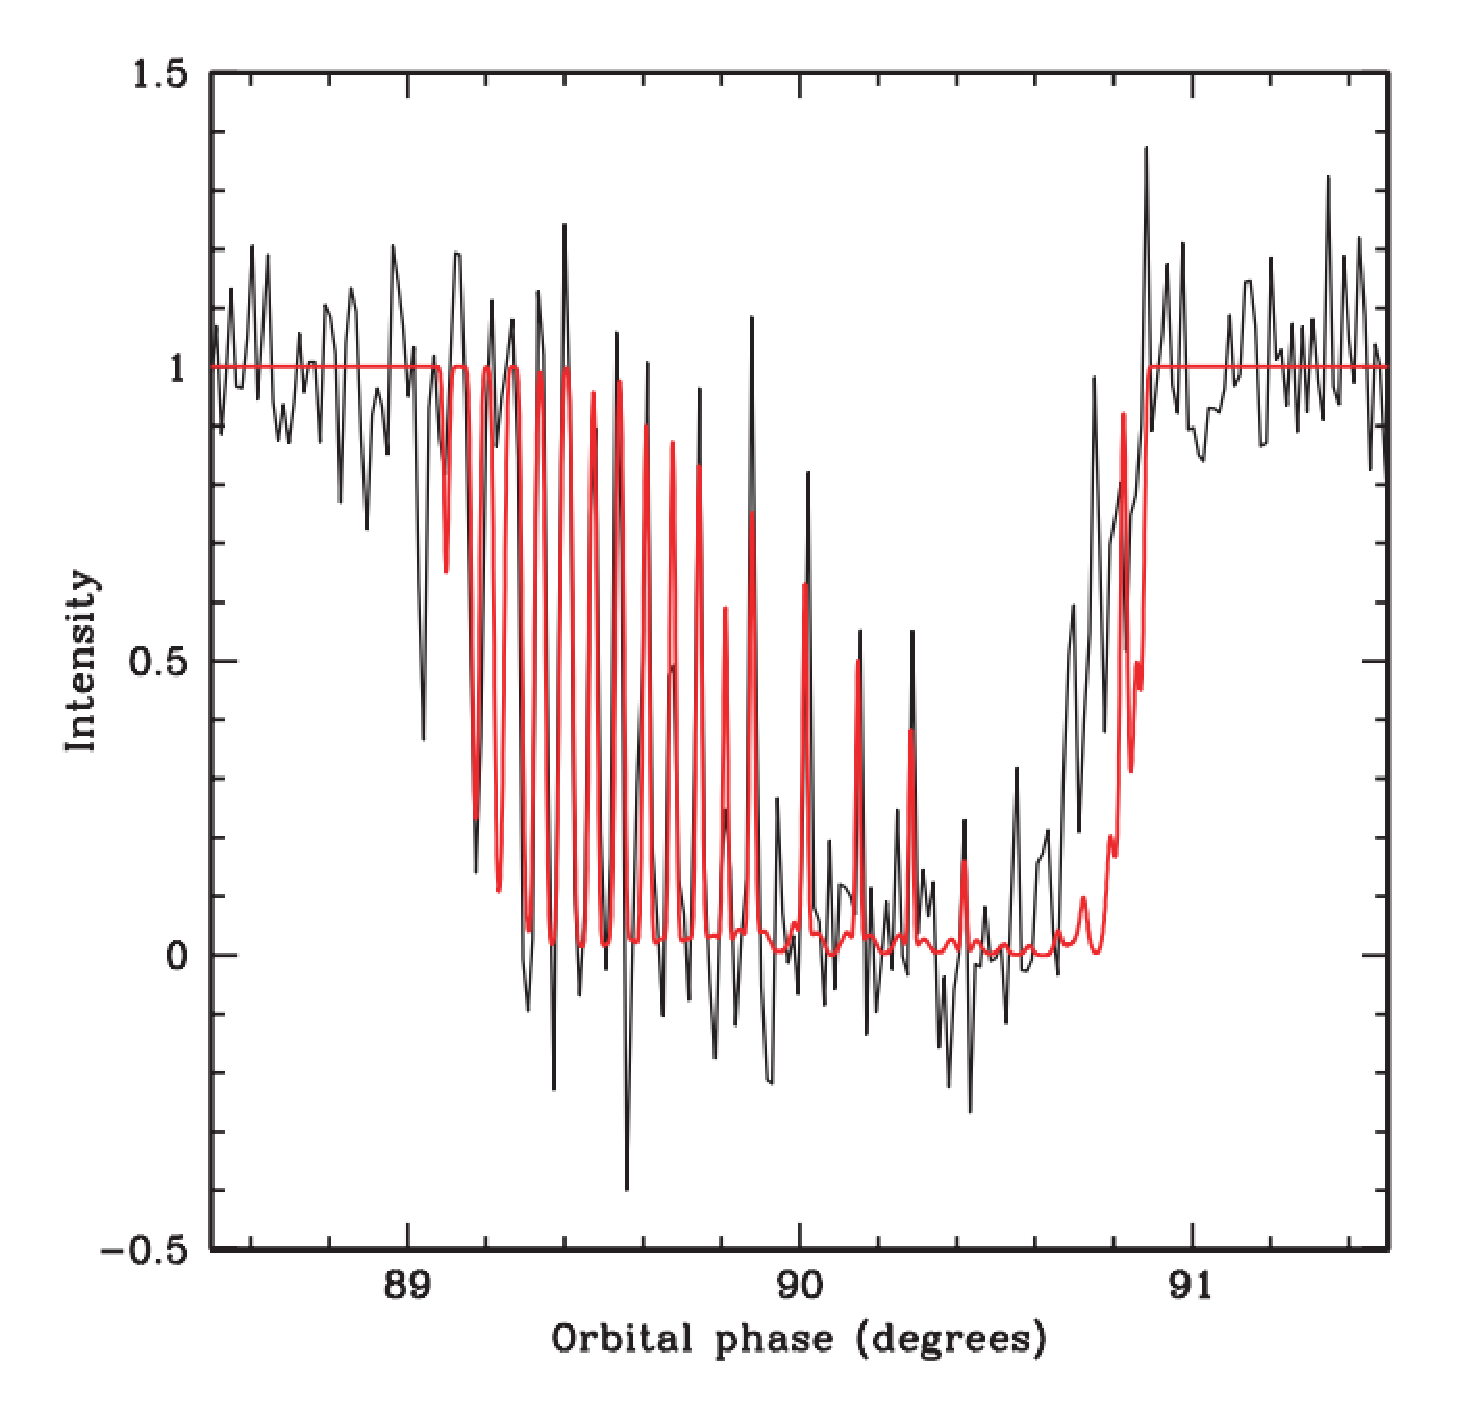
\includegraphics[width=3.4in]{fig15.eps} 
		\caption{—Comparison of a simulated eclipse profile (solid line) with 800 MHz
data by \cite{Lyut05} }
		\label{fig3}
	\end{center}
\end{figure}
% CUP work flow only accepts EPS -- not PDF, JPG, etc.
\begin{figure}[H]
	\begin{center}
		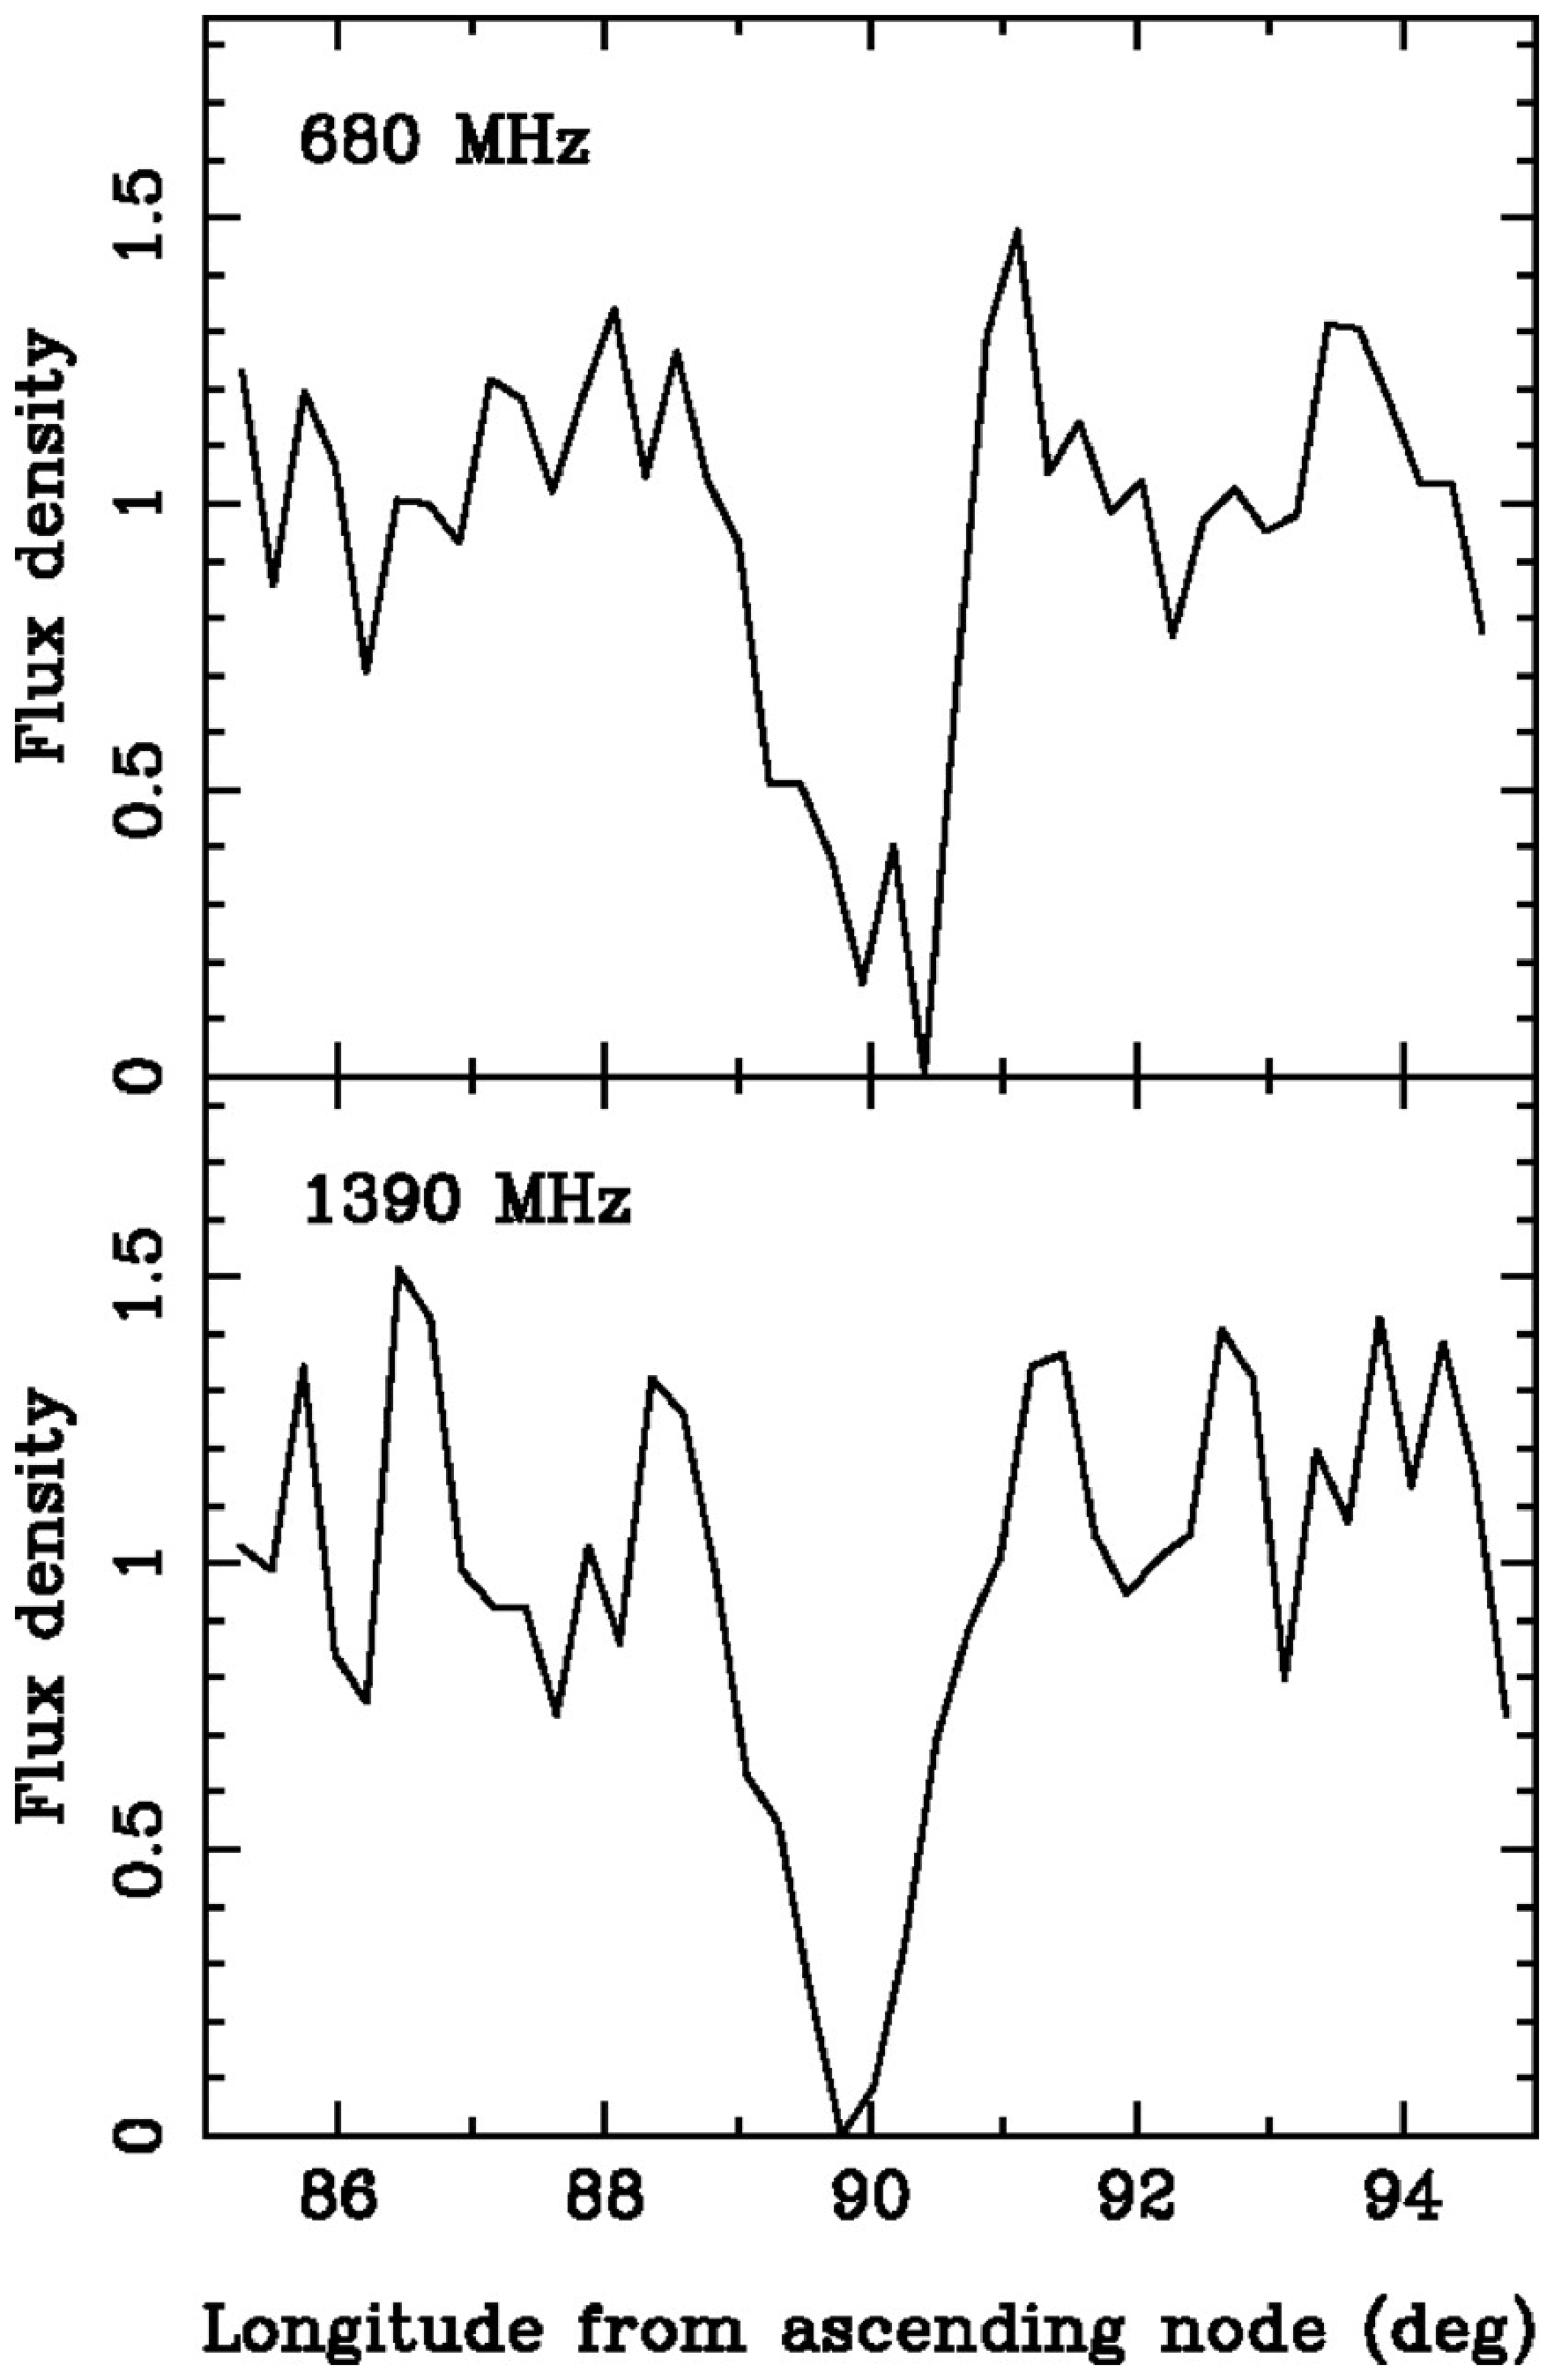
\includegraphics[width=2.4in]{fig3.eps} 
		\caption{The variation in flux density of A (in arbitrary units) at 680 and 1390 MHz, around superior conjunction (i.e., longitude 90°). The data are presented with 5-s time resolution and show the eclipse of the pulsar by the magnetosphere of B.Image and description taken from \cite{lyn04} }
		\label{fig3}
	\end{center}
\end{figure}

% CUP work flow only accepts EPS -- not PDF, JPG, etc.
\begin{figure}[H]
	\begin{center}
		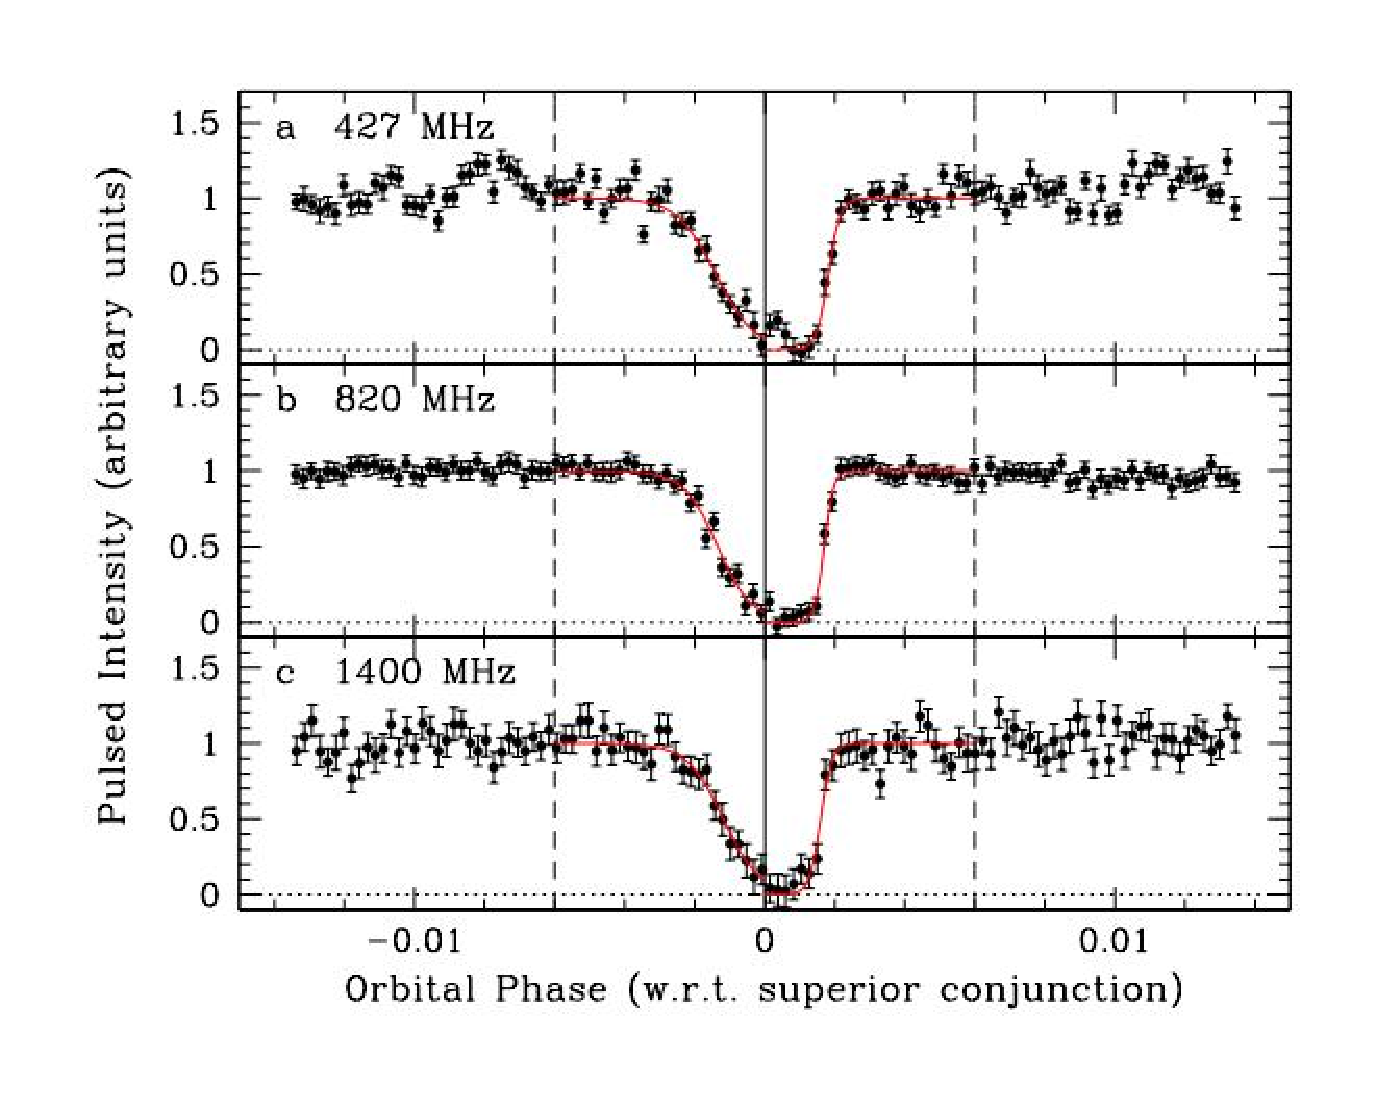
\includegraphics[width=3.4in]{fig4.eps} 
		\caption{Pulsar A eclipse light curves. Each point represents 2 s of data; the shown curve
			is 4-min in duration, centered on conjunction. The x-axes are orbital phase with respect to
			conjunction. The y-axes are pulsed flux, normalized such that the pre-eclipse flux is unity.
			The panels are for (a) 427 MHz, (b) 820 MHz, and (c) 1400 MHz. The solid vertical line
			indicates conjunction and the horizontal dotted lines show 0 flux. Vertical dashed lines at
			$\phi$ = −0.006, +0.006 indicate the range of data fitted. The best-fit ingress and egress model
			curves are shown as solid lines. Figure and its description is from \cite{kapsi04} }
		\label{fig4}
	\end{center}
\end{figure}

\cite{kapsi04} observed the eclipsing of A in further detail using measurements from the Green Bank Telescope at 427,820, and 1400 MHz.  The light curves(figure 4) obtained showed that  the eclipse ingress is longer than the eclipse egress. The observation also confirmed the eclipse model put forth by \cite{arons05} (Note that Aaron's paper was unpublished when GBT's results were published). A's wind confines B's magnetosphere on the side facing A, compressing it. While the part of B's magnetosphere opposite to the side facing A develops a magnetotail. The heating up of A's wind plasma by the bow shock developed was hypothesized to rise of synchroton absorption, leading to A's eclipse. The rotation of B's magnetosphere was held accountable for the eclipse asymmetries. It was also postulated that at frequencies around 5-10GHz, the eclipse will clear. 

\subsection{Implications for the DNS Merger Rates}

As already explained, PSR J0737-3039 has provided a rigorous testing ground for gravitation theories. However, it must be noted that the very first important result obtained from observations of stars in this system led to setting new limits on the DNS merger rates. A relativistic DNS system such as this is expected to result in a gravitational wave burst and a neutron star/black hole depending on the properties of stars in the system \cite{lipun04}. 

When PSR J0737-3039 was discovered, its lifetime was first found to be 85Myr. Since PSR B1913+16 and PSR B1534+12 were the highest contributors to merger rate calculations at that time, the lifetime and luminosity of PSR J0737-3039 was compared with these two stars. Since the lifetime of PSR B1913+16 was 300 My, PSR J0737-3039's discovery significantly affected the DNS merger rate estimates. With these considerations, \cite{b03} calculated that PSR J0737-3039 caused a decrease in DNS merger rates by one order of magnitude. So the DNS merger rate went from $10^{-5}$ year$^{-1}$ to $10^{-4}$ year$^{-1}$. This helps in getting a more informed estimate of when and where to expect gravitational waves from and becomes more important with the detection of gravitational waves by LIGO. 



\section {X-Ray}

The pulsed emission from pulsar B could no longer be detected after 2008, as reported by \cite{per10}. It was proposed that pulsar B would be visible by 2014 if a bipolar beam shape is assumed, but analysis by \cite{lom14} showed that depending on the beam shape, the pulsar B should reappear in 2034,2043, or 2066. The prevalent models were thus unable to explain the disappearance of pulsar B. Even before that, the pulse variability and eclipsing of pulsar A were attributed by \cite{lyn04} to magnetospheric-wind interactions in the pulsar system which could not be completely characterized using only radio observations. X-ray observations were thus required to study the magnetospheric properties of the pulsar binary system. 

The first X-ray observations came from Chadra's Advanced CCD Imaging Spectrometer analyzed by \cite{laugh04}. The 0.2-10 keV luminosity was found to be  $L_x = 2 \times 10^{30} erg s^{-1} $ at a distance of 0.5 kpc. The photon index was reported to be $\Gamma$=2.9$\pm$0.4. It was speculated that the X-Ray emission was coming from magnetosphere of pulsar A. Alternatively, it was proposed that relativistic winds of pulsar A and pulsar B colliding lead to X-ray emission. However, further study was required to make more definite statements about the magnetospheric properties of the pulsar system.

To further constrain the high-energy emission spectrum of the system and get a better insight into the flux variability of the source, \cite{pelli04} studied PSR J0737-3039 using XMM-Newton's European Photon Imaging Camera (EPIC). The data collected fitted well to an absorbed power-law model with $\Gamma$=3.5$_{-.03}^{+0.5}$ and an absorption of N$_H$=(7.0$\pm$2.5)$\times$10$^{20}$ cm$^{-2}$. The data also satisfied a bremsstrahlung model with a temperature of 0.5$\pm$0.1 keV and N$_H<$5$\times$10$^{20}$ cm$^{-2}$. A blackbody(BB) plus a power law(PL) model was also applied which fit to the data at $\Gamma$=2. \cite{pelli04} compared the results obtained with other millisecond pulsars and concluded that a composite spectrum was the most plausible model to go with. While the thermal component was predicted to be possibly coming form pulsar A, the non-thermal component was speculated to be from particle acceleration at the bow shocks due to magnetospheric interactions between the two pulsars as suggested by \cite{gar04}. One definite spectral model could still not be determined, though. \cite{pelli04} were also not able to get significant data on pulsating x-ray emission.

The first pulsed emission in X-rays were detected by \cite{chat07} using Chandra's High Resolution Camera (HRC-S) for observations spanning 10.5 orbits. No pulsations were observed from pulsar B. This was an important finding since now it was known that all of the X-ray emission was coming from pulsar A. The pulse profile from pulsar A was double peaked and highly modulated. The pulse profile also aligned with the radio observations, thus further confirming the timing measurements(figure 7). Contrary to the initial predictions, no orbital modulation in the X-ray emission was seen. The possibility of the X-rays coming from bow shock was thus ruled out. Although this was a big step ahead in solving the mystery of X-ray emissions in the system, no clear consensus was reached on the mechanism. 

\begin{figure}[H]
	\begin{center}
		\includegraphics[width=3.4in]{fig7.eps} 
		\caption{ X-ray pulse profile of pulsar A, obtained by folding 89 ks of Chandra
			HRC-S data with Tempo and a DE 405 timing solution. The uncertainties on each
			bin are 1$\sigma$. The pulse profile is shown twice for clarity, and a
			radio pulse profile obtained at 1.4 GHz (as presented by \cite{man05}) is plotted below(in arbitrary units) for comparison. Both profiles are folded using the radio timing solution and are therefore aligned in phase. Image and caption taken from \cite{chat07} }
		\label{fig7}
	\end{center}
\end{figure}

Important developments in the understanding of the system happened after the 2006 and 2011 observations as part of the XMM-Newton Large Programs, where ~20,000 X-ray counts were detected from the system. The duration of these observations collected about 41 orbital periods and is thus the most extensive observation of the system to date. The analysis for this data was presented by \cite{iac16}. They further confirmed the timing of pulsar A by an accuracy of 10$^{-12}$. Even though pulsar B was not visible in the radio after 2008, this observation was able to detect X-ray emission from pulsar B(figure 7). The X-ray period of pulsar B was measured to be 2.7734665(8) s, which differs by 5.7$\times$10$^{-6}$ s from the radio observations. It could be because radio ephimeris used for making the calculation was not updated after the disappearance of pulsar B. Furthermore, variations in pulsed flux and pulse profile were seen along the orbit, which is speculated to be coming from the brightening of pulsar B by energy transfer from pulsar A. 

\begin{figure}[H]
	\begin{center}
		\includegraphics[width=3.4in]{fig8.png} 
		\caption{ Background subtracted PSR B profile for the 0.15–3.0 keV energy band obtained by folding the 2011 combined EPIC-MOS and EPIC-pn data (both light curves with 10 bins—in
			black—and 20 bins—in green—are displayed) Image and caption taken from \cite{iac16} }
		\label{fig8}
	\end{center}
\end{figure}

The analysis by \cite{iac16} also gave the first evidence of flux orbital variability in the system. However, the modulation does not correlate with the pulse flux variations from pulsar A or pulsar B. It was thus hypothesized that the modulation is a result of interaction between the wind/magnetosphere of the pulsars. The possibility of X-ray emission rising due to a bow shock mechanism was also revived as result of this finding. To further study the mechanism of X-ray emission, the same data was use for spectral analysis of the system by \cite{egr17}. 

\begin{table}[]
	\centering
	\caption{A comparison of the spectral models of the system by 
	\cite{iac16}}
	\begin{figure}[H]
		\begin{center}
			\includegraphics[width=4.4in]{fig9.png} 
	%		\label{fig9}
		\end{center}
	\end{figure}

\end{table}

As pointed out by \cite{pelli08},from a theoretical standpoint, the X-ray spectrum of the system could be one of the following-
surface thermal emission+non-thermal magnetospheric emission from both stars, and orbital phase dependent bow-shock emission due to interaction of pulsar A's wind with pulsar B's magnetosphere. Until the analysis by \cite{egr17}. the leading models for X-ray emission from the system were a two-component PL+BB model and a three-component PL+2BB model. The flux calculated from 2011 data in the 0.2-3 keV range using PL+BB model was ~4.3$\times$10$^{-14}$ erg cm$^{-2}$ s$^{-1}$. These results were consistent with the 2006 data which gave a flux of ~4.0$\times$10$^{-14}$ erg cm$^{-2}$ s$^{-1}$. For the first time, observations in the Hard X-ray spectrum(4-8 keV) were observed from this system. Like the previous observation analysis, \cite{pelli08} also found that the data fit well to a BB model and a BB+PL model. However, since most of the non-thermal X-ray is coming form pulsar A, as predicted by \cite{iac16}, the BB model was not favored. It is also interesting to note that even though the data from five years of X-ray observations was analyzed, and the relativistic spin precession in this time was ~25$\deg$, no spectral variability was observed. The possibility of a bow shock from pulsar A emitting X-rays was thus ruled out once again. The source of thermal emission was narrowed down to it being coming from the polar caps of pulsar A since the pulsars are too old to be emitting intrinsic thermal radiation, as suggested by \cite{zav09}.

\begin{figure}[H]
	\begin{center}
		\includegraphics[width=3.4in]{fig10.png} 
		\caption{ Two-component model (power law plus blackbody) applied to the
			EPIC-pn data obtained in 2006 and 2011. The different colors refer to
			the different XMM-Newton orbits (black and red: 2006, green, blue, and
			cyan: 2011). Image and caption taken from \cite{egr17} }
		\label{fig9}
	\end{center}
\end{figure}

\begin{figure}[H]
	\begin{center}
		\includegraphics[width=3.4in]{fig11.png} 
		\caption{Above 2 keV, photons are not well fitted by the model.  Image taken from \cite{egr17} }
		\label{fig10}
	\end{center}
\end{figure}

The hard X-ray data is, however, not fit by either the BB or BB+PL model. This was thus attributed to Fe K$\alpha$ emissions. It is also the first Fe K$\alpha$ emission from a non accreting system. As explained by \cite{mil07}, such emissions are usually from the innermost parts of accretion disks from black holes and neutron star X-ray binaries. Thus, the a new mystery of the possibility of a gaseous disk around one of the pulsars came up. Two models have been proposed for a relic disc existing from the supernovae that led to the formation of pulsar B. The fall-back accretion model suggests that the ejected material returned after the formation of the pulsar. The second theory suggests that the disc formed as the magnetosphere of pulsar A moved through the supernovae of pulsar B. The Fe K$\alpha$ emission lines were not observed in the 2011 data, possibly due to the spin precession of pulsar B. 

Conclusively, the analysis of XMM-Newton Large Programs gave a definite measurement and limits on the X-ray emission from PSR J0737-3039. It was concluded that the BB+PL model is more favorable to the 2BB model. The possibility of a relic disk being present was also proposed due to the detection of Fe K$\alpha$ lines. To get a better constraint on the timing data, observations from NuSTAR X-ray mission have been proposed.

\section{Optical and Far Ultraviolet}

The optical emission from pulsars, if any, is usually in the form of thermal radiation from the surface of the star, and/or non-thermal radiation from the magnetosphere(synchrotron radiation). However, only eighteen pulsars have been detected in the optical spectrum, of which, only seven have a pulsed emission in the optical. As a starting point, the luminosity of a pulsar due to synchroton radiation an be estimated as being proportional to $P^{-10}$, as concluded by \cite{Pacini71} in his study of the Vela pulsar. Furthermore, the effects of duty cycle (as proposed by \cite{Pacini87}) and orbital geometry also need to be taken into account. Pulsars thus have brightness on the order of 10, and are thus very faintly visible in optical region. 

For PSR J0737-3039, the optical and UV observations followed extensive study of the system by XMM Newton in X-ray. There has been only one optical study of the system performed by Ferraro et. al . The observations by \cite{ferr12} were made using the High Resolution Camera of the Advanced Camera for Surveys (ACS) on board the Hubble Space Telescope . The X-Ray studies by \cite{Pelli08}  proposed three component model for the system- a power law and two blackbody components. The optical studies were done to confirm these findings . The images were taken using the F606W filter (roughly corresponding to Johnson's V filter) and F435W filter(roughly corresponding to Johnson's B filter). Since the pulsar is located around 4" from a bright star, the HRC cornograph was used. The detection in optical was still not possible and only upper limits were estimated. 

The pulsar proper motion was estimated by \cite{ferr12} to be $\mu_{\alpha\cos(\delta)}$=3.82$\pm$0.62 mas $yr^{-1}$ and $\mu_\delta$=2.13$\pm$0.23 mas $yr^{-1}$. The magnitude of the system in STmag magnitude system was calculated to be $m_F435W$=27.0 and $m_F606W$=28.3. Using the following relation, mag$_\lambda$=-2.5log $F{_\lambda}$ - 21.1 , the spectral flux was calculated to be F$_F435W$=8.7 $\times$ 10$^{-5}$ keV cm$^{-2}$ s$^{-1}$ and  F$_F606W$=4.2 $\times$ 10$^{-5}$ keV cm$^{-2}$ s$^{-1}$. These spectral fluxes were then used to constrain the spectral model mentioned earlier. 

To constrain the spectral model suggested by X-ray analysis, the power law and blackbody components were extended into the optical range. Only the extrapolated cold blackbody component was in agreement with the optical measurements (figure 5). The spin down luminosity of pulsar A being three orders of magnitude higher than that of B ( as discussed bt \cite{lyn04}), the optical emission is expected to be magnetospheric emission from pulsar A. From the extrapolation, it was thus concluded by \cite{ferr12} that either the pulsar A magnetosphere does not provide any contribution in the non-thermal region or there is a break at these wavelengths. The spectral model of power law and two blackbody components as predicted by the XMM-Newton data would comply with the optical study only in the case of a spectral break at low energies in the power law component. Such a spectral break was observed by \cite{Mig14} in many pulsars, and is thus a possibility. It was expected that observations in UV will be possible that will allow making better constraints on the thermal emission from the system.
\begin{figure}[H]
	\begin{center}
		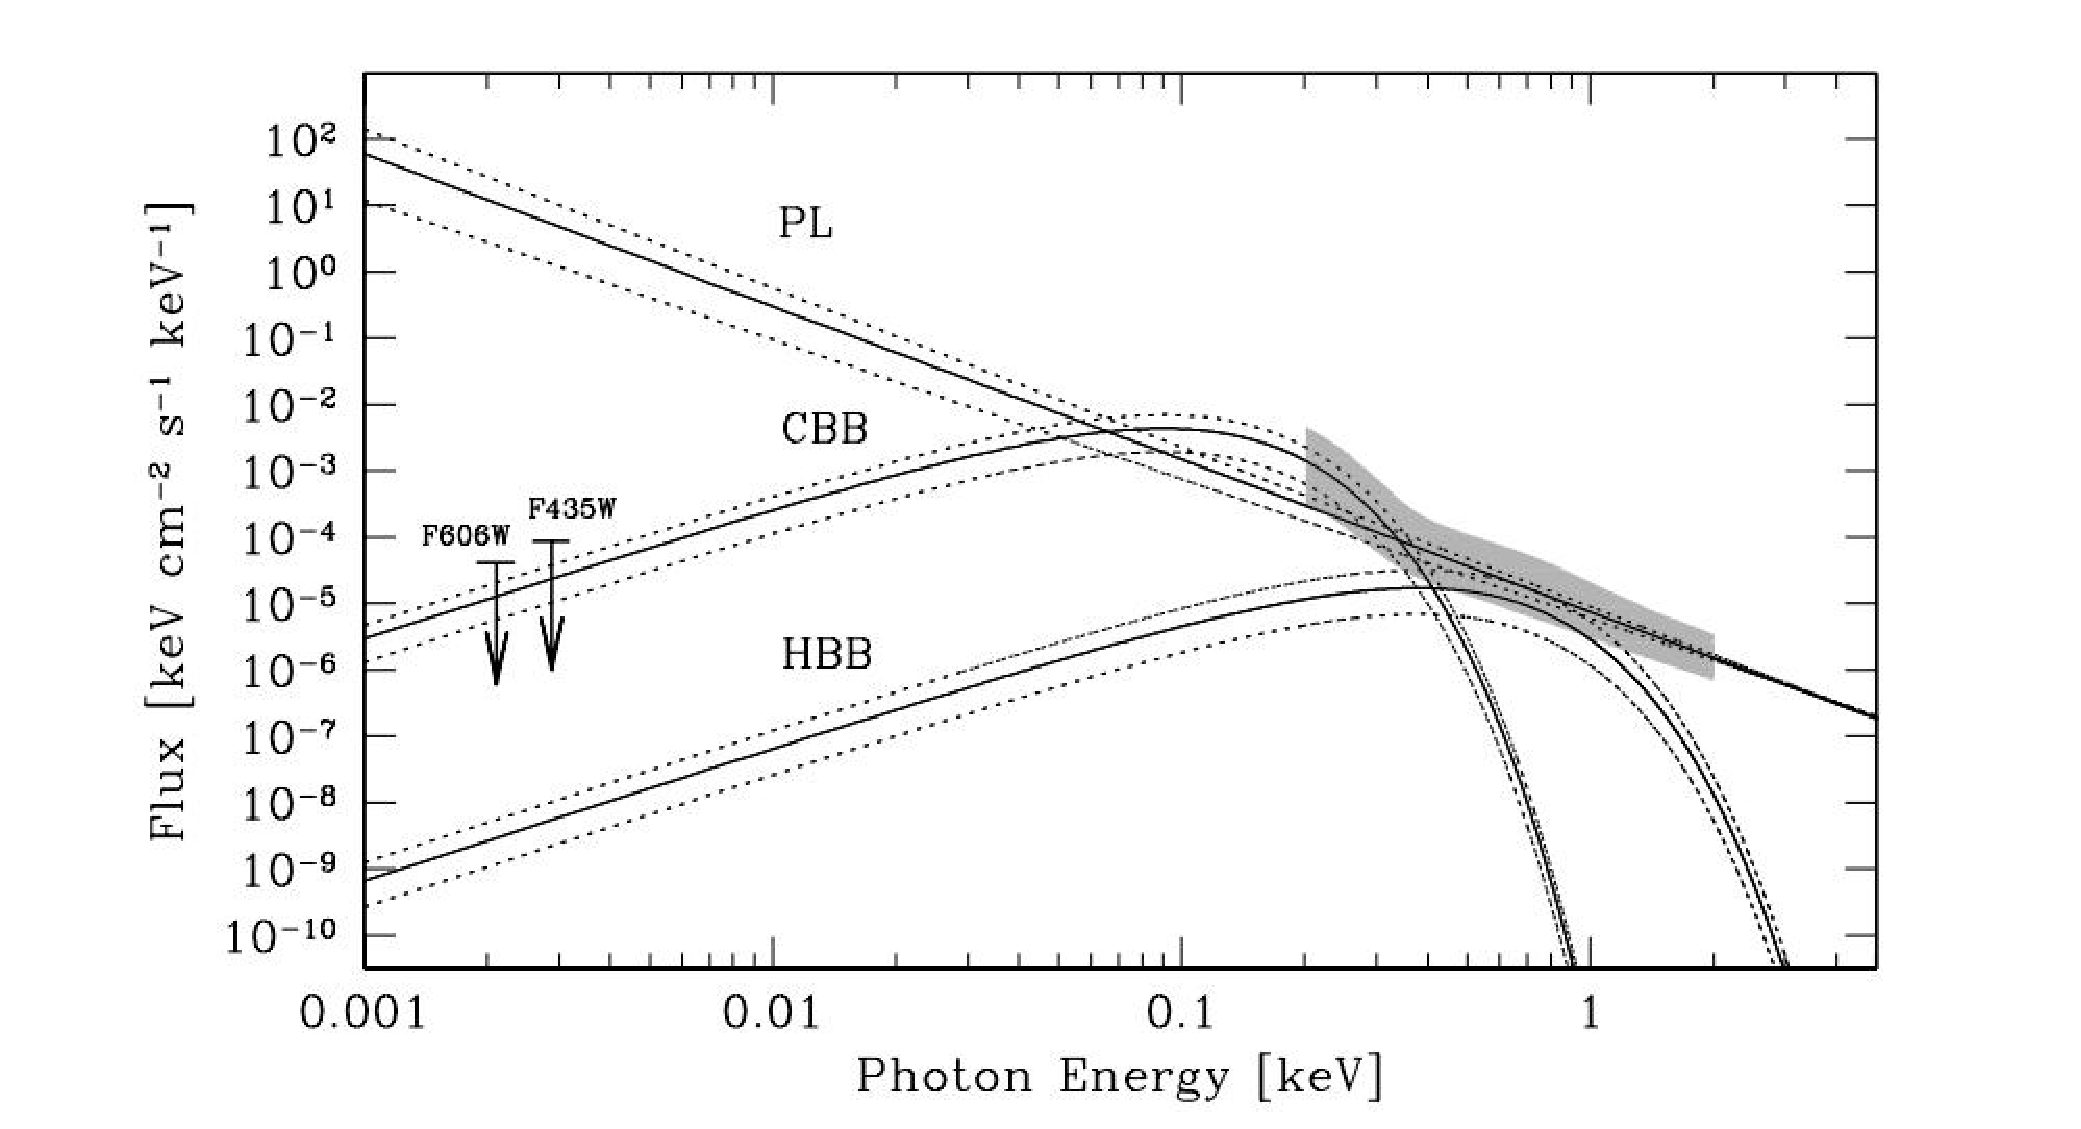
\includegraphics[width=3.4in]{fig5.eps} 
		\caption{Extrapolation into the optical regime of the model that best fits the XMM-Newton data of the pulsar system: a cooler BB and a hotter BB plus a PL. The
			solid lines are the best-fit model components, while the dot-dashed lines correspond to the 90$\%$ confidence level uncertainties of the best fit. The gray region marks the location and uncertainties of the X-ray measurements. The two arrows indicate the F435W- and F606W-band upper limits obtained from the HST data.Image and description taken from \cite{ferr12} }
		\label{fig5}
	\end{center}
\end{figure}

The system was observed in the FUV using Solar Blind Channel of ACS aboard the HST by \cite{Dur14} . Low-pass filter F125LP was used to make these observations. As with the optical analysis, the extrapolated power law component from X-Ray observations overshoots the UV measurements (figure 6). This again hints at a power law spectrum that breaks at lower energies. Additionally, after taking the observed reddening into account (E(B-V)=0.1), a temperature of 0.4 MK was obtained. However, applying this to the X-ray model yielded an emitting radius of around 33 km. It was significantly more than the expected value, and it was thus concluded that the three component spectral model predicted by X-Rays could indeed be incomplete. A final statement about the validity of the model could not be made before further observations in UV and optical are made.

\begin{figure}[H]
	\begin{center}
		\includegraphics[width=3.4in]{fig6.eps} 
		\caption{Measurements and models for the spectral flux of J0737. The unfilled
			and filled triangles show the measured and extinction-corrected FUV fluxes,
			respectively, in the F125LP and F140LP filters for E(B − V ) = 0.1. The upper
			limits in two optical filters are from \cite{ferr12}. The unabsorbed X-ray spectrum taken from \cite{Pelli08} is shown by the thick line; the dotted line shows the cold BB component from the BB+BB model for the phase-integrated X-ray spectrum. The solid and dashed lines show examples of BB models which best fit the F125LP detection for E(B − V ) = 0.1. The radii in the legend are for d = 1.1 kpc.Image and description taken from \cite{Dur14} }
		\label{fig6}
	\end{center}
\end{figure} 

\section{Gamma Rays}

The gamma ray observations of PSR J0737-3039 come from the Large Area Telescope on board the Fermi satellite and was analyzed by \cite{gui13}. The gamma ray observations of pulsar A and pulsar B were expected to provide a better constraint on the inclination angle of the magnetic axis and observer viewing angle with respect to the spin axis. There were also hopes of getting a more constrained model on the high-energy emission form the pulsar system. On scanning the data from Fermi LAT events between August 2004 and March 2012, only the pulses from pulsar A could be identified. 

The photon flux was measured to be 6$\pm3 \times 10^{-9}$ photons cm$^{-2}$ s$^{-1}$. The energy flux was measured to be 4$\pm1 \times 10^{-12}$ erg cm$^{-2}$ s$^{-1}$. The spectrum could not be modelled well enough to obtain a plausible value for photon index, so all values were reported with assuming the photon index equal to 1.3, as is common for other millisecond pulsars. Interestingly, the photon flux and energy flux of pulsar A was found to be the lowest among all millisecond pulsars. 

For gamma emission, there are two prevalent emission models to understand geometry. One is the outer gap picture(OG) where the radiation is emitted between the null charge surface and the two-pole caustic model, where the radiation is emitted from surface the the region upto 3/4th of the radius of the light cylinder. The modeled light curves as per the gamma ray observations is shown in figure 11. 
The misalignment between the spin axis and orbital momentum axis was found to be ~$\deg$. This futher confirms the theory that a small kick was imparted to the system by supernovae explosion of pulsar B, hinting that supernovae could have been caused due to an O-Ne-Mg core collapse. This was in agreement with the predictions made by  \cite{pod05}. No pulse modulations were observed in the data and it will be interesting to look for such modulations in future gamma ray analysis. 

\begin{figure}[H]
	\begin{center}
		\includegraphics[width=3.4in]{fig12.png} 
		\caption{Top: modeled light curves and γ -ray data for PSR J0737−3039A. Bottom: 1.4 GHz radio profile and best-fitting profiles. TPC light curves are shown as
pink lines and OG light curves are shown as green lines. The vertical dashed pink line and the dash-dotted green line indicate the closest approach to the magnetic axis
under the best-fit TPC and OG models, respectively. Image and caption from \cite{gui13} }
		\label{fig11}
	\end{center}
\end{figure}

\section{Conclusion}

PSR J0737-3039 was thus one of the most important double neutron star systems ever discovered owing to its unique phenomenology. The radio observations of the system led to one of the best tests for general relativity, thanks to the nearly perfectly edge-on orbital angle of the system which allowed the measurement of Shapiro delay and spin precession of pulsar B.  It also gave an insight about the formation of double neutron stars and helped in getting quantitative constraints on the stars formed as per the Roche-lobe overflow model described by \cite{dewi10}. 

The eclipsing phenomenon of pulsar A by pulsar B and the pulse modulations of pulsar B gave a new view into how magnetospheric interaction might work in similar systems. X-ray observations of the system by XMM-Newton and Chandra helped in getting a more quantitative understanding by providing composite spectrum models to explain the magnetospheric emissions in the system. Observations in optical, ultraviolet, and gamma make it one of the most extensively studied double neutron star system which has both of the stars detected as pulsars. 

With the discovery of new double neutron star systems such as the PSR J1757–1854 by \cite{cam17} could help in getting answers to the questions that PSR J0737-3039 left answered. The observations from PSR J0737-3039 would also provide constraints to parameters for the more recently discovered double pulsar systems and is mostly treated as a model system for double pulsar systems. 





\begin{thebibliography}{}


\bibitem[Arons et al. (2005)]{arons05} Arons, J., C. Backer, D., Spitkovsky, A., M. Kaspi, V., 2005. 95.
\bibitem[Breton et al. (2008)]{bret08} Breton, R.P., Kaspi, V.M., Kramer, M., McLaughlin, M.A., Lyutikov, M., Ransom, S.M., Stairs, I.H., Ferdman, R.D., Camilo, F., Possenti, A., 2008. Science 321, 104–107.
\bibitem[Burgay et al. (2003)]{b03} Burgay, M., N. D’Amico, A. Possenti, R. N. Manchester, A. G. Lyne, B. C. Joshi, M. A. McLaughlin, et al. 2003. Nature 426 (6966): 531–33. https://doi.org/10.1038/nature02124.
\bibitem[Cameron et al. (2017)]{cam17} Cameron, A.D., Champion, D.J., Kramer, M., Bailes, M., Barr, E.D., Bassa, C.G., Bhandari, S., Bhat, N.D.R., Burgay, M., Burke-Spolaor, S., Eatough, R.P., Flynn, C.M.L., Freire, P.C.C., Jameson, A., Johnston, S., Karuppusamy, R., Keith, M.J., Levin, L., Lorimer, D.R., Lyne, A.G., McLaughlin, M.A., Ng, C., Petroff, E., Possenti, A., Ridolfi, A., Stappers, B.W., van Straten, W., Tauris, T.M., Tiburzi, C., Wex, N., 2017. Proceedings of the International Astronomical Union 13, 134–137.
\bibitem[Chatterjee et al. (2007)]{chat07} Chatterjee, S., Gaensler, B.M., Melatos, A., Brisken, W.F., Stappers, B.W., 2007. The Astrophysical Journal 670, 1301.
\bibitem[Dewi et. al (2010)]{dewi10} Dewi, J.D.M., 2010. New Astronomy Reviews, Proceedings: A Life With Stars 54, 145–147.
\bibitem[Durant et al. (2014)]{Dur14} Durant, M., Kargaltsev, O., Pavlov, G.G., 2014. The Astrophysical Journal 783, L22.
\bibitem[Egron et al. (2017)]{egr17} Egron, E., Pellizzoni, A., Pollock, A., Iacolina, M.N., Ikhsanov, N.R., Possenti, A., Marongiu, M., 2017. The Astrophysical Journal 838, 120.
\bibitem[Ferraro et. al (2012)]{ferr12} Ferraro, F.R., Mignani, R.P., Pallanca, C., Dalessandro, E., Lanzoni, B., Pellizzoni, A., Possenti, A., Burgay, M., Camilo, F., D’Amico, N., Lyne, A.G., Kramer, M., Manchester, R.N., 2012. The Astrophysical Journal 749, 84.
\bibitem[Granot and Mészáros (2004)]{gar04} Granot, J., Mészáros, P., 2004. The Astrophysical Journal 609, L17.
\bibitem[Guillemot et al. (2013)]{gui13}Guillemot, L., Kramer, M., Johnson, T.J., Craig, H.A., Romani, R.W., Venter, C., Harding, A.K., Ferdman, R.D., Stairs, I.H., Kerr, M., 2013. ApJ 768, 169.
\bibitem[Iacolina et al. (2016)]{iac16} Iacolina, M.N., Pellizzoni, A., Egron, E., Possenti, A., Breton, R., Lyutikov, M., Kramer, M., Burgay, M., Motta, S.E., Luca, A.D., Tiengo, A., 2016. The Astrophysical Journal 824, 87.
\bibitem[James et al. (2016)]{james16}  James Justin Condon, Scott M. Ransom, 2016. 6 Pulsars‣ Essential Radio Astronomy [WWW Document]. URL https://www.cv.nrao.edu/~sransom/web/Ch6.html (accessed 10.17.18).
\bibitem[Kaspi et al., (2004)]{kapsi04} Kaspi, V.M., Ransom, S.M., Backer, D.C., Ramachandran, R., Demorest, P., Arons, J., Spitkovsky, A., 2004. The Astrophysical Journal 613, L137–L140.

\bibitem[Kramer and Wex (2009)]{kwex09} Kramer, M., Wex, N., 2009. Class. Quantum Grav. 26, 073001.

\bibitem[Lipunov (2004)]{lipun04} Lipunov, V.M., 2004. arXiv:astro-ph/0406502.
\bibitem[Lomiashvili and Lyutikov (2014)]{lom14} Lomiashvili, D., Lyutikov, M., 2014. Mon Not R Astron Soc 441, 690–714.
\bibitem[Lyne (2006)]{lyn06} Lyne, A.G., 2006. Chinese Journal of Astronomy and Astrophysics Supplement 6, 162.
\bibitem[Lyne (2010)]{lyn10} Lyne, A.G., 2010. New Astronomy Reviews, Proceedings: A Life With Stars 54, 135–139.
\bibitem[Lyne et al. (2004)]{lyn04} Lyne, A.G., Burgay, M., Kramer, M., Possenti, A., Manchester, R.N., Camilo, F., McLaughlin, M.A., Lorimer, D.R., D’Amico, N., Joshi, B.C., Reynolds, J., Freire, P.C.C., 2004. Science 303, 1153–1157.
\bibitem[Lyutikov and Thompson, (2005)]{Lyut05} Lyutikov, M., Thompson, C., 2005. ApJ 634, 1223.
\bibitem[Manchester et al. (2005)]{man05} Manchester, R.N., Lyne, A.G., Burgay, M., Kramer, M., Possenti, A., Camilo, F., Hotan, A.W., McLaughlin, M.A., Lorimer, D.R., D’Amico, N., Joshi, B.C., Reynolds, J.E., Freire, P.C.C., 2005. Binary Radio Pulsars 328, 67.
\bibitem[McLaughlin et al. (2004)]{laugh04} McLaughlin, M.A., Camilo, F., Burgay, M., D’Amico, N., Joshi, B.C., Kramer, M., Lorimer, D.R., Lyne, A.G., Manchester, R.N., Possenti, A., 2004. The Astrophysical Journal 605, L41–L44.
\bibitem[Mignani et al. (2014)]{Mig14} Mignani, R.P., Corongiu, A., Pallanca, C., Oates, S.R., Yershov, V.N., Breeveld, A.A., Page, M.J., Ferraro, F.R., Possenti, A., Jackson, A.C., 2014. Monthly Notices of the Royal Astronomical Society 443, 2223–2241.
\bibitem[Miller (2007)]{mil07} Miller, J.M., 2007. Annual Review of Astronomy and Astrophysics 45, 441–479.
\bibitem[Pacini (1971)]{Pacini71} Pacini, F., 1971. The Astrophysical Journal 163, L17–L19.
\bibitem[Pacini et. al (1987)]{Pacini87} Pacini, F., Salvati, M., 1987. The Astrophysical Journal 321, 447.
\bibitem[Pellizzoni et al. (2004)]{pelli04} Pellizzoni, A., Luca, A.D., Mereghetti, S., Tiengo, A., Mattana, F., Caraveo, P., Tavani, M., n.d. 612, 4.
\bibitem[Pellizzoni et al. (2008)]{Pelli08} Pellizzoni, A., Tiengo, A., De Luca, A., Esposito, P., Mereghetti, S., 2008. The Astrophysical Journal 679, 664–674.
\bibitem[Pellizzoni et al. (2008)]{pelli08} Pellizzoni, A., Tiengo, A., Luca, A.D., Esposito, P., Mereghetti, S., 2008. ApJ 679, 664.
\bibitem[Perera et al. (2010)]{per10} Perera, B.B.P., McLaughlin, M.A., Kramer, M., Stairs, I.H., Ferdman, R.D., Freire, P.C.C., Possenti, A., Breton, R.P., Manchester, R.N., Burgay, M., Lyne, A.G., Camilo, F., 2010. ApJ 721, 1193.
\bibitem[Podsiadlowski et al. (2005)]{pod05} Podsiadlowski, P., Dewi, J.D.M., Lesaffre, P., Miller, J.C., Newton, W.G., Stone, J.R., 2005. Monthly Notices of the Royal Astronomical Society 361, 1243-1249.
\bibitem[Zavlin (2009)]{zav09} Zavlin, V.E., 2009. Theory of Radiative Transfer in Neutron Star Atmospheres and Its Applications. Presented at the Astrophysics and Space Science Library, p. 181.
\end{thebibliography}


\end{document}
